\documentclass{standalone}
\usepackage{tikz}
\begin{document}
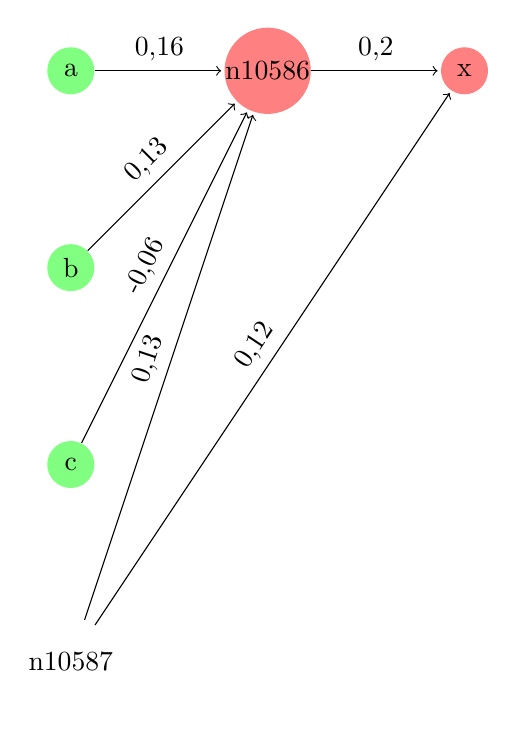
\begin{tikzpicture}[shorten >=1pt,->,draw=black!,node distance=2.5cm]
\tikzstyle{neuron}=[circle,fill=black!25,minimum size=17pt,inner sep=0pt]
\tikzstyle{constant}=[neuron, fill=white!50];
\tikzstyle{sigmoid}=[neuron, fill=red!50];
\tikzstyle{identity}=[neuron, fill=green!50];
\node [identity] (a) {a};
\node [identity,below of=a] (b) {b};
\node [identity,below of=b] (c) {c};
\node [constant,below of=c] (n10587) {n10587};
\node [sigmoid,right of=a] (n10586) {n10586};
\node [sigmoid,right of=n10586] (x) {x};
\path[every node/.style={sloped,anchor=south,auto=false}]
(n10586) edge node {0,2} (x)
(n10587) edge node {0,12} (x)
(n10587) edge node {0,13} (n10586)
(b) edge node {0,13} (n10586)
(a) edge node {0,16} (n10586)
(c) edge node {-0,06} (n10586)
;\end{tikzpicture}
\end{document}